\documentclass{article}
\usepackage{blindtext}
\usepackage{amsmath}
\usepackage{amssymb}
\usepackage{amsmath}
\usepackage[utf8]{inputenc}
\usepackage{bbm}
\usepackage[margin=1in]{geometry} % set margins
\usepackage{subcaption} % allows for subfigures
\usepackage{graphicx} % allow inclusion of figures/photos/pdfs
\usepackage{harvard} % sets citation style
\usepackage{setspace} % allows changes between 
% \doublespacing \singlespacing \onehalfspacing
\onehalfspacing
\graphicspath{{./figure/}}
\usepackage[justification=centering]{caption}
\usepackage{cancel}
\usepackage{mathrsfs}

\usepackage{Sweave}
\begin{document}
\Sconcordance{concordance:Dilgin_Where_to_Spend.tex:Dilgin_Where_to_Spend.Rnw:%
1 19 1 1 0 12 1 1 2 1 0 6 1 1 2 2 1 1 3 1 0 1 5 3 0 1 3 1 0 12 1 1 2 1 %
1 1 2 1 7 6 0 1 1 1 7 6 0 1 2 2 1 1 2 4 0 1 3 3 1}

	\title{Where to Spend the Money? A Survey Experiment on Electoral Institutions and Party Expenditure at the District Level}
	\author{Tolgahan Dilgin}
	\date{12/12/2018}
	\maketitle
	
\begin{abstract}
   This paper is part of dissertation research that examines the impact of electoral institutions on how political parties choose to engage in vote buying practices at the district level. Regardless of electoral rules, parties tend to concentrate their vote buying spending in the most competitive districts as opposed to party strongholds in order to maximize their electoral gains. This research argues that Proportional Representation (PR) systems enable political parties distribute their vote buying activities more evenly between party strongholds and competitive districts in comparison to Single Member District (SMD) systems. In the face of difficulty in testing this theory empirically, the paper takes advantage of the unique political structure of Mexico, which uses both SMD and PR systems in its elections. The survey experiment with Mexican students -who are exposed to both of the systems- seems to provide evidence consistent with paper's main theoretical claim.
\end{abstract}

\section{Introduction}

\begin{Schunk}
\begin{Sinput}
> library(ggplot2)
> library(reshape2)
> library(dplyr)
> library(data.table)
> library(stargazer)
> require(knitr)
> require(kableExtra)
> data = read.csv("Mexican_Data_Combined.csv") 
> subdata = as.data.frame(data)
> subdata = subdata[subdata$Actual.Total>=90000 & subdata$Actual.Total<=100000,]
> #subset the columns that we want to use to analyze Question 12
> subdata_12 = select(subdata, Respondent_ID, Institution_Type, P12_Distrito_1, P12_Distrito_2, P12_Distrito_3, P12_Distrito_4, P12_Distrito_5, P12_Distrito_6, P12_Distrito_7, P12_Distrito_8, P12_Distrito_9)
> #then to make the graph we need to change Districts 1-9 to there corresponding competitiveness level
> 
> #rearrange data, # I use the melt function because we want the column names to be on the x-axis. We want to exlude anything that is not a district. 
> subdata_12.melt = melt(subdata_12, id=c("Respondent_ID", "Institution_Type")) 
> #Rename the districts to level of competitiveness and Institution Type to English abbreviation.
> subdata_12.melt$variable = as.character(subdata_12.melt$variable)
> subdata_12.melt$Institution_Type = as.character(subdata_12.melt$Institution_Type)
> subdata_12.melt$variable[subdata_12.melt$variable == "P12_Distrito_1"] = "-.3"
> subdata_12.melt$variable[subdata_12.melt$variable == "P12_Distrito_2"] = "-.4"
> subdata_12.melt$variable[subdata_12.melt$variable == "P12_Distrito_3"] = "-.5"
> subdata_12.melt$variable[subdata_12.melt$variable == "P12_Distrito_4"] = "-.1"
> subdata_12.melt$variable[subdata_12.melt$variable == "P12_Distrito_5"] = "0"
> subdata_12.melt$variable[subdata_12.melt$variable == "P12_Distrito_6"] = "-.1"
> subdata_12.melt$variable[subdata_12.melt$variable == "P12_Distrito_7"] = "-.5"
> subdata_12.melt$variable[subdata_12.melt$variable == "P12_Distrito_8"] = "-.4"
> subdata_12.melt$variable[subdata_12.melt$variable == "P12_Distrito_9"] = "-.3"
> subdata_12.melt$Institution_Type[subdata_12.melt$Institution_Type == "RP"] = "PR"
> subdata_12.melt$Institution_Type[subdata_12.melt$Institution_Type == "MR"] = "SMD"
> subdata_12.melt = subdata_12.melt[complete.cases(subdata_12.melt), ] #to remove NAs
> subdata_12.melt = transform(subdata_12.melt, variable = as.numeric(variable)) #change variable from character to numerical
> Competitive = c()
> for (i in subdata_12.melt$variable) {
+   if (i == "0" | i == "-0.1") {
+     Competitive = c(Competitive, 1)
+   } else {
+     Competitive = c(Competitive, 0)
+   }
+ }
> Binary_IT = c()
> for (i in subdata_12.melt$Institution_Type) {
+   if (i == "SMD") {
+     Binary_IT = c(Binary_IT, 1)
+   } else {
+     Binary_IT = c(Binary_IT, 0)
+   }
+ }
> subdata_12.melt = cbind(subdata_12.melt, Binary_IT, Competitive)
> names(subdata_12.melt)[3]<-"Competitiveness"
> names(subdata_12.melt)[4]<-"District_Spending"
> ggplot(subdata_12.melt, aes(x = Competitiveness, y = District_Spending, color = Institution_Type)) + geom_jitter() + geom_smooth(method='lm', se = FALSE) + coord_cartesian(ylim = c(4000,20000)) + ggtitle("Mexican Students (ITAM)") + labs(y="District Spending", x = "Margin of Vote", color = "Electoral System") + scale_x_continuous(breaks = c(-.5, -.4, -.3, -.2, -.1, 0))
> 
\end{Sinput}
\end{Schunk}
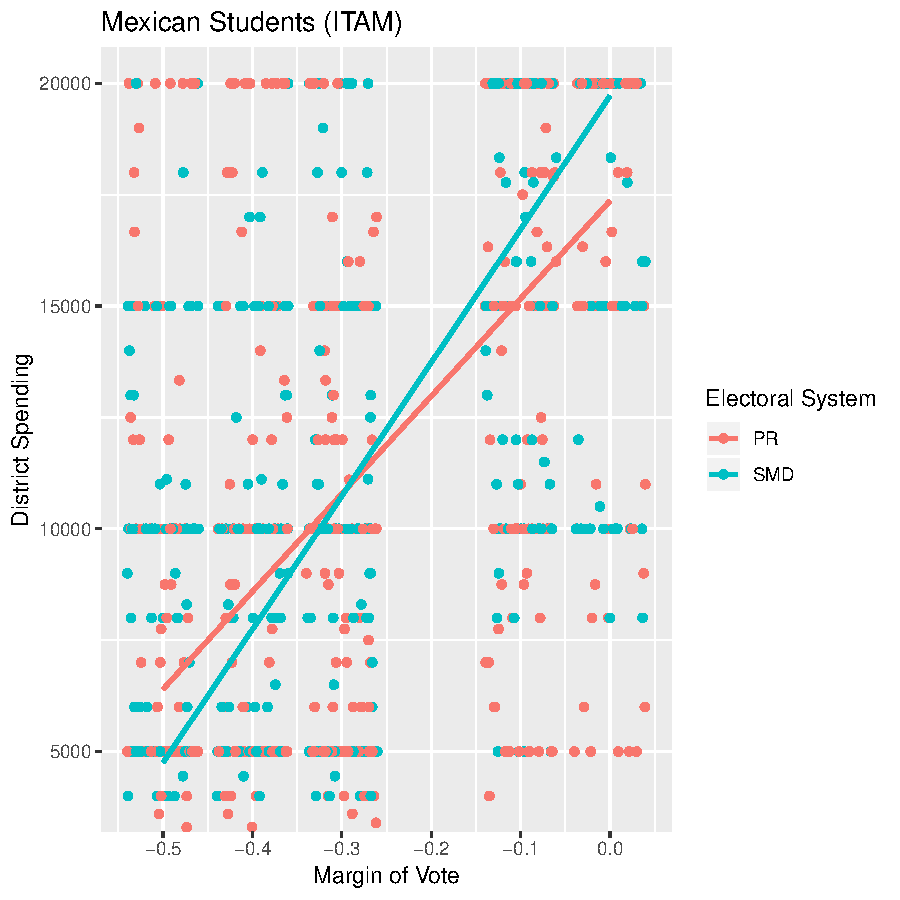
\includegraphics{Dilgin_Where_to_Spend-001}


\begin{Schunk}
\begin{Soutput}
Call:
lm(formula = District_Spending ~ Competitiveness, data = InstitutionTypeSubSet$SMD)

Coefficients:
    (Intercept)  Competitiveness  
          19721            29941  
\end{Soutput}
\begin{Soutput}
Call:
lm(formula = District_Spending ~ Competitiveness, data = InstitutionTypeSubSet$PR)

Coefficients:
    (Intercept)  Competitiveness  
          17365            21932  
\end{Soutput}
\begin{Soutput}
Call:
lm(formula = District_Spending ~ Competitive + Binary_IT + Competitive * 
    Binary_IT, data = subdata_12.melt)

Residuals:
   Min     1Q Median     3Q    Max 
-18617  -5299  -1458   3353  41780 

Coefficients:
                      Estimate Std. Error t value Pr(>|t|)    
(Intercept)             8219.6      366.3  22.437  < 2e-16 ***
Competitive             8427.3      634.5  13.281  < 2e-16 ***
Binary_IT               -920.9      510.9  -1.802  0.07173 .  
Competitive:Binary_IT   2890.8      885.0   3.267  0.00112 ** 
---
Signif. codes:  0 '***' 0.001 '**' 0.01 '*' 0.05 '.' 0.1 ' ' 1

Residual standard error: 7454 on 1274 degrees of freedom
Multiple R-squared:  0.2871,	Adjusted R-squared:  0.2854 
F-statistic:   171 on 3 and 1274 DF,  p-value: < 2.2e-16
\end{Soutput}
\end{Schunk}

\begin{Schunk}
\begin{Soutput}
                       Estimate Std. Error   t value     Pr(>|t|)
(Intercept)           8219.5604   366.3415 22.436881 3.162220e-94
Competitive           8427.2850   634.5221 13.281311 8.527904e-38
Binary_IT             -920.8937   510.9388 -1.802356 7.172564e-02
Competitive:Binary_IT 2890.8474   884.9719  3.266598 1.117467e-03
\end{Soutput}
\end{Schunk}

r, echo=FALSE}
library(broom)
tidy(Mexico_model)
```
